% !TEX root = ../thesis.tex

\chapter{Introduction}

\begin{itemize}
  \item "lakes"
  \item \la
  \begin{itemize}
    \item what?
    \begin{itemize}
      \item comparative research of lake, but still ``closed system''
    \end{itemize}
    \item why?
    \begin{itemize}
      \item
    \end{itemize}
    \item how?
    \begin{itemize}
      \item MATLAB
    \end{itemize}
    \item why important?
    \begin{itemize}
      \item
    \end{itemize}
  \end{itemize}
    \item relevance of lakes to global process such as the carbon cycle \citep{cole2007plumbing}.
  \item challenges
  \begin{itemize}
    \item large scale data
    \item live analysis
    \begin{itemize}
      \item indefinite large data sets
    \end{itemize}
    \item advanced analysis
    \begin{itemize}
      \item model chains
      \item composite models
      \item model chains
    \end{itemize}
    \item GDP etc.
    \begin{itemize}
      \item based on OGC services
      \item WPS\dots
    \end{itemize}
  \end{itemize}
  \item problems
  \begin{itemize}
    \item non interoperable
    \item thus can not incorporated into another model chains
    \item \citep{downing2006global}
  \end{itemize}
  \item solutions

  \item build upon \ac{OGC} standards such as \acrocitep{CSW}{ogc:csw}, \acrocitep{WPS}{ogc:wps}, \acrocitep{WMS}{ogc:wms} and \acrocitep{WCS}{ogc:csw}
  \item such as the USGS’s \ac{GDP}\footnote{\url{http://cida.usgs.gov/gdp/}}
  \item \citep[e.g. \la\footnote{\url{https://github.com/GLEON/Lake-Analyzer}}, see][]{read2011derivation})
\end{itemize}

Recent research has highlighted the relevance of lakes to global process such as the carbon cycle \citep{cole2007plumbing}.
Ecological studies on lakes have historically taken advantage of the ``closed system'' bounds to delineate a simplified ecosystem, but analyses that are formulated to answer societally relevant questions often must scale this single system science approach to hundreds, thousands, or millions of lakes \citep{downing2006global}.
Therefore systems must be developed that can aggregate, analyze, and ultimately interpret hydrological data at large scales. Additionally, these analytical systems must be able to easily couple lake features with supporting data that define, for example, catchment properties, local climate, and anthropomorphic stressors.
These data products are readily available as national coverages that can either be sampled and turned into model parameters, or turned into model drivers if they are time series products.

This work shall evaluate the existing tools \citep[e.g. \la\footnote{\url{https://github.com/GLEON/Lake-Analyzer}}, see][]{read2011derivation}), data models and the modeling frameworks used by USGS CIDA\footnote{\url{http://cida.usgs.gov/}}.
Modeling runs are based on online data brokers (such as the USGS’s \ac{GDP}\footnote{\url{http://cida.usgs.gov/gdp/}}) build upon \ac{OGC} standards such as \acrocitep{CSW}{ogc:csw}, \acrocitep{WPS}{ogc:wps}, \acrocitep{WMS}{ogc:wms} and \acrocitep{WCS}{ogc:csw}, but still rely on local algorithms, which comprise functionality for statistical quality assurance and quality control as well as the calculation of various metrics related to the physical state of the lakes (often linked with ecosystem function or disturbance). Building standardized and flexible infrastructure for analyzing foundational data used by domain scientists is an important challenge given legacy and heterogeneous architectures.
Therefore building on the existing infrastructure and corresponding demands of the use case shall be considered.

One approach for a scalable system is to move the modeling to a web-based processing framework, which should rely on public and interoperable standards in the given use case.
Web processing allows to chain data brokers with translators, models, and eventually post-hoc analysis of model runs.
This chain provides specific information products to the user.
Considering the amount of data (and future process scaling needs), such an analysis must be conducted in a streaming manner, i.e. the processing should start before the last chunk of data comes in, and the output should also be available in parts before the processing has completely finished to reduce the lag for domain users of the system.
Existing approaches to this problem shall be critically evaluated.

This thesis work comprises the evaluation, design and prototypical implementation of a lake analysis chain for live sensor data.
This includes the evaluation of existing data models (mainly CSV/TSV) and a standardized way to convert existing domain specific applications written in MatLab\footnote{\url{http://www.mathworks.de/products/matlab/}} into streaming web services (possibly WPS algorithms) in favor of the currently used non standardized web frontend\footnote{\url{http://lakeanalyzer.gleon.org/}}.

\paragraph*{Research Questions}
\begin{itemize}
  \item How can large scale hydrological data be processed in a service-based processing chain?
  \item Do available web-processing interface definitions support a live data streaming scenario, what is missing?
  \item Can real-time data be integrated into the processing chain for a constant (streamed) analysis?
  \item How does the developed architecture perform in practical test with 1000s and 10000s of lake features?
  \item How can continued statistical quality assurance and quality control in the application area of lake ecology be modeled in a web service chain?
  \item Do existing standards (data models and service interfaces for data warehousing, processing and visualization) support a streaming analysis chain? What is missing?
  \item How can spatial dependencies between streamed features be considered?
  \item How can a analysis language commonly used by domain experts (in this case MATLAB) be easily deployed in a web based processing chain?
\end{itemize}

\chapter{\la}
\la is tool to compute key characteristics of lakes with regards to the lake's thermal stratification and its stability. It analyzes times series data of water temperature measurements obtained using instrumented lake buoys as well as wind speed observations using the lake's bathymetric areas with respect to depth and optional salinity measurements to improve water density calculations. It promotes comparative lake research, which is made possible due to the increased temporal resolution and spatial extent of lake measurements by offering a consistent methodology that can be applied to many types of lakes \citep{read2011derivation}.

\la allows to predict biological phenomenon (e.g. the likelihood of nutrient upwelling that can cause algal blooms), explain phenological pattern in aquatic organisms, control and monitor the state of a lake as well as to improve the quality of models by comparing their outputs to the physical state of the lake that is computed by the \la.

Besides a raw data output as \ac{CSV}, the \la features a visualizations of the produces stratification and mixing indices, which can be seen in \cref{fig:la:outputs:1}: Lake Number \citep[see \cref{fig:la:out:Ln,fig:la:out:SLn},][]{imberger1990}, metalimnion extent (see \cref{fig:la:out:metaT,fig:la:out:metaB,fig:la:out:SmetaT,fig:la:out:SmetaB}), Brunt-Väisälä buoyancy frequency (see \cref{fig:la:out:N2,fig:la:out:SN2}), mode-1 vertical seiche period \citep[see \cref{fig:la:out:T1,fig:la:out:ST1},][]{monismith1986}, Wedderburn Number \citep[see \cref{fig:la:out:W,fig:la:out:SW},][]{thompson1980}, thermocline depth (see \cref{fig:la:out:thermD,fig:la:out:SthermD}), $u^{*}$ (wind stress introduced water friction velocity, see \cref{fig:la:out:uSt,fig:la:out:SuSt}) and Schmidt Stability \citep[see \cref{fig:la:out:St},][]{schmidt1928,hutchinson1957,idso1973}. The \la is able to error check and/or down sample input time series and also outputs wind speed (\cref{fig:la:out:wndSpd}) and water temperature (\cref{fig:la:out:wTemp}).

% !TEX root = ../thesis.tex

\def\lafigsize{.491\linewidth}
\def\lafigdesc{Visualization of outputs created by the \la based on an example data set of the Sparkling Lake, WI, USA}
\begin{figure}[!htb]
  \centering
  \begin{subfigure}{\lafigsize}
    \caption{\label{fig:la:out:Ln}Lake Number}
    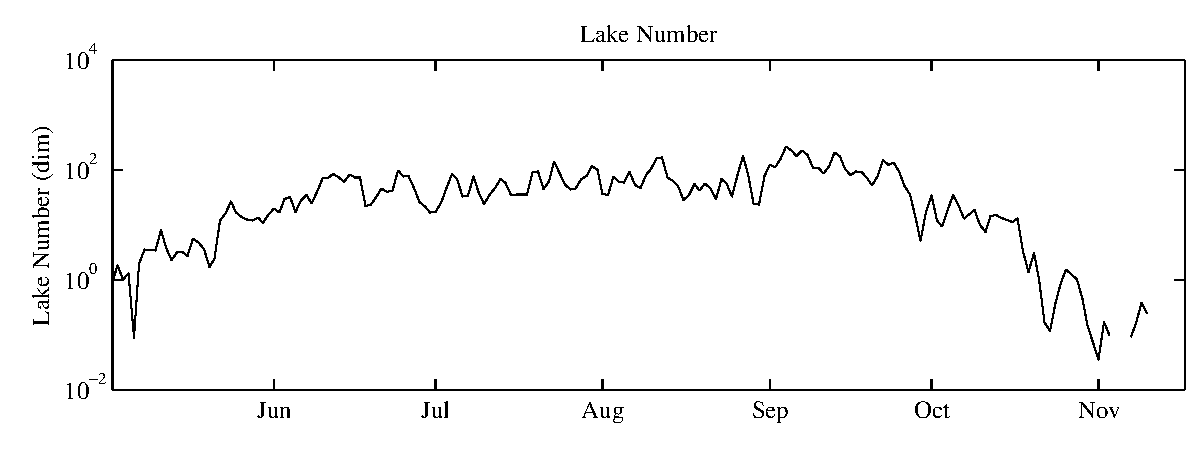
\includegraphics[width = \linewidth]{figures/Sparkling_Ln.pdf}
  \end{subfigure}
  \begin{subfigure}{\lafigsize}
    \caption{\label{fig:la:out:SLn}Seasonal Lake Number}
    \includegraphics[width = \linewidth]{figures/Sparkling_SLn.pdf}
  \end{subfigure}
  \begin{subfigure}{\lafigsize}
    \caption{\label{fig:la:out:metaT}Metalimnion Top}
    \includegraphics[width = \linewidth]{figures/Sparkling_metaT.pdf}
  \end{subfigure}
  \begin{subfigure}{\lafigsize}
    \caption{\label{fig:la:out:metaB}Metalimnion Bottom}
    \includegraphics[width = \linewidth]{figures/Sparkling_metaB.pdf}
  \end{subfigure}
  \begin{subfigure}{\lafigsize}
    \caption{\label{fig:la:out:SmetaT}Seasonal Metalimnion Top}
    \includegraphics[width = \linewidth]{figures/Sparkling_SmetaT.pdf}
  \end{subfigure}
  \begin{subfigure}{\lafigsize}
    \caption{\label{fig:la:out:SmetaB}Seasonal Metalimnion Bottom}
    \includegraphics[width = \linewidth]{figures/Sparkling_SmetaB.pdf}
  \end{subfigure}
  \begin{subfigure}{\lafigsize}
    \caption{\label{fig:la:out:N2}Buoyancy Frequency}
    \includegraphics[width = \linewidth]{figures/Sparkling_N2.pdf}
  \end{subfigure}
  \begin{subfigure}{\lafigsize}
    \caption{\label{fig:la:out:SN2}Seasonal Buoyancy Frequency}
    \includegraphics[width = \linewidth]{figures/Sparkling_SN2.pdf}
  \end{subfigure}
  \begin{subfigure}{\lafigsize}
    \caption{\label{fig:la:out:T1}Mode-1 Vertical Seiche Period}
    \includegraphics[width = \linewidth]{figures/Sparkling_T1.pdf}
  \end{subfigure}
  \begin{subfigure}{\lafigsize}
    \caption{\label{fig:la:out:ST1}Seasonal Mode-1 Vertical Seiche Period}
    \includegraphics[width = \linewidth]{figures/Sparkling_ST1.pdf}
  \end{subfigure}
  \caption[\lafigdesc.]{\label{fig:la:outputs:1}\lafigdesc{} \emph{(continued on \cpageref{fig:la:outputs:2})}.}
\end{figure}
\begin{figure}
  \ContinuedFloat\centering\captionsetup{list=no}
  \begin{subfigure}{\lafigsize}
    \caption{\label{fig:la:out:W}Wedderburn Number}
    \includegraphics[width = \linewidth]{figures/Sparkling_W.pdf}
  \end{subfigure}
  \begin{subfigure}{\lafigsize}
    \caption{\label{fig:la:out:SW}Seasonal Wedderburn Number}
    \includegraphics[width = \linewidth]{figures/Sparkling_SW.pdf}
  \end{subfigure}
  \begin{subfigure}{\lafigsize}
    \caption{\label{fig:la:out:thermD}Thermocline Depth}
    \includegraphics[width = \linewidth]{figures/Sparkling_thermD.pdf}
  \end{subfigure}
  \begin{subfigure}{\lafigsize}
    \caption{\label{fig:la:out:SthermD}Seasonal Thermocline Depth}
    \includegraphics[width = \linewidth]{figures/Sparkling_SthermD.pdf}
  \end{subfigure}
  \begin{subfigure}{\lafigsize}
    \caption{\label{fig:la:out:uSt}$u^{*}$}
    \includegraphics[width = \linewidth]{figures/Sparkling_uSt.pdf}
  \end{subfigure}
  \begin{subfigure}{\lafigsize}
    \caption{\label{fig:la:out:SuSt}Seasonal $u^{*}$}
    \includegraphics[width = \linewidth]{figures/Sparkling_SuSt.pdf}
  \end{subfigure}
  \begin{subfigure}{\lafigsize}
    \caption{\label{fig:la:out:St}Schmidt Stability}
    \includegraphics[width = \linewidth]{figures/Sparkling_St.pdf}
  \end{subfigure}
  \begin{subfigure}{\lafigsize}
    \caption{\label{fig:la:out:wndSpd}Wind Speed}
    \includegraphics[width = \linewidth]{figures/Sparkling_wndSpd.pdf}
  \end{subfigure}
  \begin{subfigure}{\lafigsize}
    \caption{\label{fig:la:out:wTemp}Water Temperature}
    \includegraphics[width = \linewidth]{figures/Sparkling_wTemp.pdf}
  \end{subfigure}
  \caption{\label{fig:la:outputs:2}\lafigdesc.}
\end{figure}
